%!TEX program = xelatex
%%%%%%%%%%%%%%%%%%%%%%%%%%%%%%%%%%%%%%%%%%%%%%%%%%%%%%%%%%%%%%%%%%%%%%%%%%%%%%%%%
%
% This is a very basic template for mathematical presentations using LaTeX and beamer, aimed at University of Edinburgh students on the Honours Analysis course 2017-2018, for their "Skills" presentations.
%
% This template is just to get you started and to see what the possibilities are.  There is no required format, and you are free to use, discard, edit as much as you like.  I've put in some mathematical content to demonstrate the very basics of LaTeX.  Clearly, you will need to change this.
%
% Except for a few structural comments, I don't comment on the LaTeX itself.  If you have used it before, most of what you know should apply as usual.  If you have not, have a look at the source code, the output, and experiment with editing the code and see what happens.  Most LaTeX code is pretty intuitive, e.g. the command to produce an alpha is \alpha, the command for an integral sign is \int, etc.  You can learn an awful lot by guesswork, trial and error, and google.  
%
% The percent signs "%" are comment signs, and instruct LaTeX to ignore everything following the sign on the same line.  They can be used to comment on the code.
%
%%%%%%%%%%%%%%%%%%%%%%%%%%%%%%%%%%%%%%%%%%%%%%%%%%%%%%%%%%%%%%%%%%%%%%%%%%%%%%%%
%
% The following lines are the preamble.  They help LaTeX set-up the document, but do not print anything yet.

\documentclass[usenames,dvipsnames]{ctexbeamer}		% This tells LaTeX the document will be a "beamer" presentation

\usetheme{Madrid}		% Sets basic formatting.  Lots of options, google "beamer themes"

\usepackage{xcolor}
\usepackage{tikz}

\usepackage[colorlinks,linkcolor=blue]{hyperref}
\usetikzlibrary {arrows.meta,backgrounds,fit,positioning}
\definecolor{forestgreen}{rgb}{0.13, 0.55, 0.13}
%%% logo
\pgfdeclareimage[height=0.8cm]{logo}{./logo.png}
\logo{\pgfuseimage{logo}}
%\logo{\vspace*{-0.3cm}\pgfuseimage{logo}}


\usecolortheme{dolphin}	% Sets the colour scheme.  Lots of options, google "beamer color themes"

%\setbeamertemplate{navigation symbols}{}
% Manually changes one piece of formatting.  See what the difference is by commenting this line out.

\date{}	% Insert the date of your presentation. \today gives an unsurprising automatic date.

\title[String]{SA}	% Insert your title.  Depending on the theme you choose above, a "short title" might be useful, as it will appear on the footer of each slide.

\author[calabash\_boy]{calabash\_boy} % Insert your name

\date{\today}

\newcommand{\redP}{{\color{red}\#}}

\begin{document} 	% Let's begin

% Presentations come in slide frames.  You have to tell LaTeX when to start a frame, and when to end the frame.  The most common error beginners make with beamer is forgetting the \end{frame} command.	

\begin{frame}	

\titlepage	% Prints a title page populated with the information given in the preamble
	
\end{frame}		

\begin{frame}{后缀数组}

\begin{block}{定义}

\textbf{后缀$S[i]$}:$S[i] = S[i, |S|]$。

\textbf{字典序}:对于两个字符串$S$和$T$,从左到右找到第一个不同的字母,谁的字母小,谁的字典序就小。特殊的,如果$S$为$T$的前缀,认为$S < T$。即空字符最小。

\pause

\textbf{后缀排序}:将所有后缀$S[i]$看作独立的串,放在一起按照字典序进行升序排序。

\textbf{后缀排名$rk[i]$}:$rk[i]$表示后缀$S[i]$在后缀排序中的排名,即他是第几小的后缀。

\textbf{后缀数组$sa[i]$}:$sa[i]$表示排名第$i$小的后缀。

\color{red}{$rk[sa[i]] = i$}
\end{block}
    
\end{frame}

\begin{frame}{求后缀数组1}

\begin{block}{Naive Sort法}

用二分Hash写一个比较字典序的cmp函数,然后直接调sort。

复杂度$O(n\log^{2}{n})$

\pause
Hash检测次数高达$n\log^{2}{n}$,非常容易冲突。且复杂度过高。

\end{block}

\end{frame}

\begin{frame}{求后缀数组2}
\begin{block}{前缀倍增法}
思路:将比较字典序的二分求LCP转化为倍增求LCP。

\pause

首先等效的认为在字符串的末尾增添无限个空字符$\emptyset$。

\vbox{}
定义$S(i, k) = S[i, i + 2^{k} - 1]$,即以$i$位置开头,长度为$2^k$的子串。

后缀$S[i]$与$S[j]$的字典序关系等价于$S(i, \infty)$ 与$S(j, \infty)$的字典序关系。

事实上,只需要将$S(i, \lceil log_{2}{n} \rceil)$,$i = 1, 2, \cdots, n$排序即可。
\end{block}    
\end{frame}

\begin{frame}{求后缀数组2}

\begin{block}{前缀倍增法}

于是便可以倍增的进行排序,假设当前已经得到了$S(i,k)$的排序结果,即$rk[S(i,k)]$与$sa[S(i,k)]$,思考如何利用它们排序$S(i,k+1)$。

\pause

\vbox{}
由于$S(i, k+1)$是由$S(i,k)$和$S(i + 2^k, k)$前后拼接而成。

因此比较$S(i,k+1)$与$S(j,k+1)$字典序可以转化为先比较$S(i,k)$与$S(j,k)$,再比较$S(i+2^k,k)$与$S(j+2^k,k)$。

\vbox{}
因此可以将$S(i,k+1)$看作一个两位数,高位是$rk[S(i,k)]$,低位是$rk[S(i+2^k,k)]$。
\end{block}

\end{frame}

\begin{frame}{两位数的排序}

\begin{block}{一位数的排序}

有一组一位数,将他们排序只需要一个桶数组辅助就可以完成。

复杂度$O(n)$。

\end{block}

\pause

\begin{block}{两位数的排序}

有一组两位数,可以用$\{A_i,B_i\}$表示,将他们排序时,需要先按照高位排序,高位相同时,按照低位排序。此过程为基数排序。

复杂度$O(n)$。
\end{block}
\end{frame}

\begin{frame}{基数排序}

\begin{block}{基数排序}
基数排序的过程可以简单理解:

1. 首先统计$cntA[x]$,表示高位$A = x$的数字有多少个。于是可以确定第$i$个数字的最终排名一定在范围$\textbf{(}\sum_{x=1}^{x<A_i}cntA[x], \sum_{x=1}^{x \leq A_i}cntA[x]\textbf{]}$内,记为$(SumA[A_i-1], SumA[A_i]]$。即完成了数字的分块,以及完成了块与块之间的排序。

\vbox{}
2. 接下来需要确定每个块($A=x$)内数字的顺序,问题变成排序一位数:按照低位$B$从大到小,依次地领取排名$SumA[x], SumA[x]-1, \cdots,SumA[x-1] + 1$。因此这一步需要事先对把所有数字按照低位排序。
\end{block}
    
\end{frame}

\begin{frame}{求后缀数组2}

\begin{block}{前缀倍增法}

复杂度分析:

算法需要运行$\log{n}$轮。每一轮使用基数排序,复杂度为$O(n)$。

整体复杂度为$O(n\log{n})$。

\end{block}
    
\end{frame}

\begin{frame}{求后缀数组3}
    
\begin{block}{DC3法}
将所有后缀按照开头下标Mod 3分类:{\color{blue}后缀1},{\color{forestgreen}后缀2},{\color{red}后缀0}。

首先将所有{\color{blue}后缀1},{\color{forestgreen}后缀2}排序,然后加入{\color{red}后缀0}归并,得到完整的排序。
\begin{figure}
    \centering
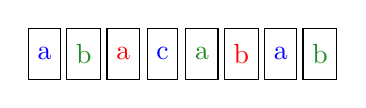
\begin{tikzpicture}[minimum height = 6.5mm]

\node (c1) at (0,0) [draw]{\color{blue}a};
\node (c2) at (0.5,0) [draw]{\color{forestgreen}b};
\node (c3) at (1,0) [draw]{\color{red}a};
\node (c4) at (1.5,0) [draw]{\color{blue}c};
\node (c5) at (2.0,0) [draw]{\color{forestgreen}a};
\node (c6) at (2.5,0) [draw]{\color{red}b};
\node (c7) at (3.0,0) [draw]{\color{blue}a};
\node (c8) at (3.5,0) [draw]{\color{forestgreen}b};

\end{tikzpicture}
\end{figure}

\end{block}
\end{frame}

\begin{frame}{求后缀数组3}
    
\begin{block}{DC3法}
1. 排序{\color{blue}后缀1},{\color{forestgreen}后缀2}
\begin{figure}
    \centering
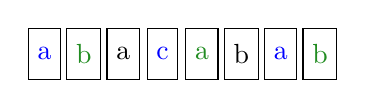
\begin{tikzpicture}[minimum height = 6.5mm]

\node (c1) at (0,0) [draw]{\color{blue}a};
\node (c2) at (0.5,0) [draw]{\color{forestgreen}b};
\node (c3) at (1,0) [draw]{a};
\node (c4) at (1.5,0) [draw]{\color{blue}c};
\node (c5) at (2.0,0) [draw]{\color{forestgreen}a};
\node (c6) at (2.5,0) [draw]{b};
\node (c7) at (3.0,0) [draw]{\color{blue}a};
\node (c8) at (3.5,0) [draw]{\color{forestgreen}b};

\end{tikzpicture}
\end{figure}

注意到所有{\color{blue}后缀1}都是$\textbf{S[1]}$的后缀,且开头位置下标差都是3的倍数。
同理,所有{\color{forestgreen}后缀2}都是$\textbf{S[2]}$的后缀。

\pause

因此我们可以用如下方法处理,进行递归:

首先,如果$S[1]$或者$S[2]$的长度不是3的倍数,则在其后分别补0到3的倍数长度。如果是3的倍数,依然需要补3个0。

\pause

然后将$S[1]$和$S[2]$前后拼接。

\begin{figure}
    \centering
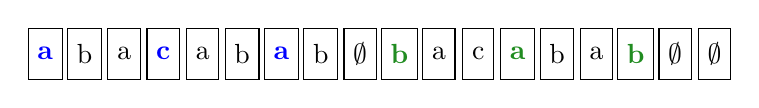
\begin{tikzpicture}[minimum height = 6.5mm]

\node (c1) at (0,0) [draw]{\color{blue}\textbf{a}};
\node (c2) at (0.5,0) [draw]{b};
\node (c3) at (1,0) [draw]{a};
\node (c4) at (1.5,0) [draw]{\color{blue}\textbf{c}};
\node (c5) at (2.0,0) [draw]{a};
\node (c6) at (2.5,0) [draw]{b};
\node (c7) at (3.0,0) [draw]{\color{blue}\textbf{a}};
\node (c8) at (3.5,0) [draw]{b};
\node (c9) at (4.0,0) [draw]{$\emptyset$};

\node (c22) at (4.5,0) [draw]{\color{forestgreen}\textbf{b}};
\node (c23) at (5,0) [draw]{a};
\node (c24) at (5.5,0) [draw]{c};
\node (c25) at (6.0,0) [draw]{\color{forestgreen}\textbf{a}};
\node (c26) at (6.5,0) [draw]{b};
\node (c27) at (7.0,0) [draw]{a};
\node (c28) at (7.5,0) [draw]{\color{forestgreen}\textbf{b}};
\node (c29) at (8.0,0) [draw]{$\emptyset$};
\node (c210) at (8.5,0) [draw]{$\emptyset$};

\end{tikzpicture}
\end{figure}

\pause
问题转化为排序$T$的所有$Mod3 = 1$位置{\color{blue}后}{\color{forestgreen}缀}。
\end{block}
\end{frame}

\begin{frame}{求后缀数组3}
    
\begin{block}{DC3法}

将每3个位置打包在一起,打包之后每个块可以看作一个三位数。
\begin{figure}
    \centering
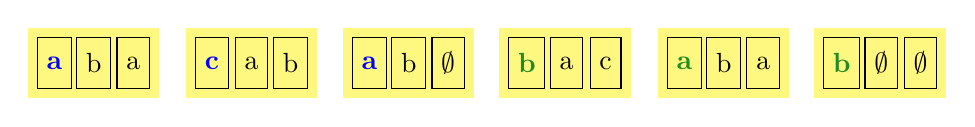
\begin{tikzpicture}[minimum height = 6.5mm]

\node (c1) at (0,0) [draw]{\color{blue}\textbf{a}};
\node (c2) at (0.5,0) [draw]{b};
\node (c3) at (1,0) [draw]{a};
\begin{scope}[on background layer]
\node [fill=yellow!50, fit=(c1) (c2) (c3)] {};
\end{scope}
\node (c4) at (2.0,0) [draw]{\color{blue}\textbf{c}};
\node (c5) at (2.5,0) [draw]{a};
\node (c6) at (3.0,0) [draw]{b};
\begin{scope}[on background layer]
\node [fill=yellow!50, fit=(c4) (c5) (c6)] {};
\end{scope}
\node (c7) at (4.0,0) [draw]{\color{blue}\textbf{a}};
\node (c8) at (4.5,0) [draw]{b};
\node (c9) at (5.0,0) [draw]{$\emptyset$};
\begin{scope}[on background layer]
\node [fill=yellow!50, fit=(c7) (c8) (c9)] {};
\end{scope}

\node (c22) at (6.0,0) [draw]{\color{forestgreen}\textbf{b}};
\node (c23) at (6.5,0) [draw]{a};
\node (c24) at (7.0,0) [draw]{c};
\begin{scope}[on background layer]
\node [fill=yellow!50, fit=(c22) (c23) (c24)] {};
\end{scope}
\node (c25) at (8.0,0) [draw]{\color{forestgreen}\textbf{a}};
\node (c26) at (8.5,0) [draw]{b};
\node (c27) at (9.0,0) [draw]{a};
\begin{scope}[on background layer]
\node [fill=yellow!50, fit=(c25) (c26) (c27)] {};
\end{scope}
\node (c28) at (10.0,0) [draw]{\color{forestgreen}\textbf{b}};
\node (c29) at (10.5,0) [draw]{$\emptyset$};
\node (c210) at (11.0,0) [draw]{$\emptyset$};
\begin{scope}[on background layer]
\node [fill=yellow!50, fit=(c28) (c29) (c210)] {};
\end{scope}

\end{tikzpicture}
\end{figure}

使用基数排序将这些三位数排序。

\begin{figure}
    \centering
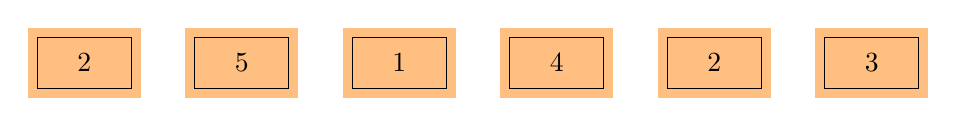
\begin{tikzpicture}[minimum height = 6.5mm]

\node (c2) at (0.5,0) [draw]{\;\;\;\;2\;\;\;\;};
\begin{scope}[on background layer]
\node [fill=orange!50, fit=(c2)] {};
\end{scope}

\node (c5) at (2.5,0) [draw]{\;\;\;\;5\;\;\;\;};
\begin{scope}[on background layer]
\node [fill=orange!50, fit=(c5)] {};
\end{scope}

\node (c8) at (4.5,0) [draw]{\;\;\;\;1\;\;\;\;};
\begin{scope}[on background layer]
\node [fill=orange!50, fit=(c8)] {};
\end{scope}

\node (c23) at (6.5,0) [draw]{\;\;\;\;4\;\;\;\;};
\begin{scope}[on background layer]
\node [fill=orange!50, fit=(c23)] {};
\end{scope}

\node (c26) at (8.5,0) [draw]{\;\;\;\;2\;\;\;\;};
\begin{scope}[on background layer]
\node [fill=orange!50, fit=(c26)] {};
\end{scope}

\node (c29) at (10.5,0) [draw]{\;\;\;\;3\;\;\;\;};
\begin{scope}[on background layer]
\node [fill=orange!50, fit=(c29)] {};
\end{scope}

\end{tikzpicture}
\end{figure}

因此排序所有$T$的所有$Mod3 = 1$位置{\color{blue}后}{\color{forestgreen}缀}转变为对{\color{orange!50}$T'=251423$}进行后缀排序。

\pause

进行递归。
\end{block}
\end{frame}

\begin{frame}{求后缀数组3}

\begin{block}{DC3法}
2. 对所有{\color{red}后缀0}排序。

\begin{figure}
    \centering
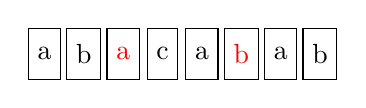
\begin{tikzpicture}[minimum height = 6.5mm]

\node (c1) at (0,0) [draw]{a};
\node (c2) at (0.5,0) [draw]{b};
\node (c3) at (1,0) [draw]{\color{red}a};
\node (c4) at (1.5,0) [draw]{c};
\node (c5) at (2.0,0) [draw]{a};
\node (c6) at (2.5,0) [draw]{\color{red}b};
\node (c7) at (3.0,0) [draw]{a};
\node (c8) at (3.5,0) [draw]{b};

\end{tikzpicture}
\end{figure}

每个{\color{red}后缀0}可以表示为${\color{red}S[3k,n]} = S[3k] + {\color{blue}S[3k+1, n]}$。即变成一个字母和一个{\color{blue}后缀1}拼接而成,可以看作一个两位数,可以使用基数排序。
\end{block}
    
\end{frame}

\begin{frame}{求后缀数组3}

\begin{block}{DC3法}
3. 将排序过的{\color{red}后缀0}与排序过的{\color{blue}后\color{forestgreen}缀\color{blue}1\color{forestgreen}2}进行归并。

\pause

\vbox{}
3.1. 如何比较{\color{red}后缀0}与{\color{blue}后缀1}:

${\color{red}S[3k,n]} = S[3k] + {\color{blue}S[3k+1,n]}$

${\color{blue}S[3p+1,n]} = S[3p+1] + {\color{forestgreen}S[3p+2,n]}$

{\color{blue}后缀1}与{\color{forestgreen}后缀2}的相对顺序已知,因此可以看作两位数$O(1)$完成比较。

\pause

\vbox{}

3.2. 如何比较{\color{red}后缀0}与{\color{forestgreen}后缀2}:

${\color{red}S[3k,n]} = S[3k] + S[3k + 1] + {\color{forestgreen}S[3k+2,n]}$

${\color{forestgreen}S[3p+2,n]} = S[3p+2] + S[3p+3] + {\color{blue}S[3p+4,n]}$

同理,可以看作三位数$O(1)$完成比较。
\end{block}
    
\end{frame}

\begin{frame}{求后缀数组3}

\begin{block}{DC3法}

复杂度$T(n) = T(\frac{2n}{3}) + O(n)$。

于是复杂度为$$O(n + \frac{2}{3}n + (\frac{2}{3})^2n + \cdots)) 
= O(\frac{n}{1-\frac{2}{3}}) 
= O(3n)$$

由于基数排序天然自带大常数,整个算法的常数会达到接近20。实际表现只比倍增优秀一点点。
\end{block}
\end{frame}

\begin{frame}{求后缀数组4}
    
\begin{block}{SA-IS}

略。小常数$O(n)$。

\end{block}
\end{frame}

\begin{frame}{后缀数组性质}

\begin{block}{LCP}

设有一组排序过的字符串$A = [A_1, A_2, \cdots, A_n]$。

如何快速的求任意$A_i$与$A_j$的LCP?

\pause

\vbox{}
“区间可加性”:对于任意的$k\in [i,j]$,$LCP(A_i, A_j) = LCP(LCP(A_i,A_k), LCP(A_k,A_j)) = min(LCP(A_i, A_k), LCP(A_k, A_j))$。

\pause
进而,$LCP(A_i, A_j) = min(LCP(A_i, A_{i+1}), LCP(A_{i+1}, A_{i+2}),\cdots, LCP(A_{j-1}, A_{j}))$。

证明:
\pause
\begin{figure}
    \centering
    
\includegraphics[width=0.95\textwidth]{./emo.png}
\end{figure}

\end{block}
\end{frame}

\begin{frame}{证明}

\begin{block}{1. $LCP(A_i, A_k) \neq LCP(A_k, A_j)$}

\begin{figure}
    \centering
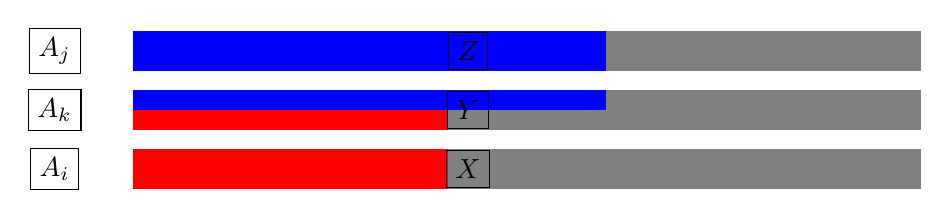
\begin{tikzpicture}
\node at (-1,0.25) [draw] {$A_i$};
\fill [gray]  (0,0) rectangle (10, 0.5);

\fill [red, very thick] (0,0) rectangle (4, 0.5);

\node at (4.25, 0.25) [draw] {$X$};

\node at (-1,1) [draw] {$A_k$};
\fill [gray]  (0,0.75) rectangle (10, 1.25);

\fill [red, very thick] (0, 0.75) rectangle (4, 1);
\fill [blue, very thick] (0,1) rectangle (6, 1.25);

\node at (4.25, 1) [draw] {$Y$};

\node at (-1,1.75) [draw] {$A_j$};
\fill [gray]  (0,1.5) rectangle (10, 2);

\fill [blue, very thick] (0, 1.5) rectangle (6, 2);

\node at (4.25, 1.75) [draw] {$Z$};
\end{tikzpicture}
\end{figure}

由于$X \neq Y$,$Y = Z$,因此$X \neq Z$。即$LCP(A_i, A_j) = LCP(A_i, A_k) = min(LCP(A_i, A_k), LCP(A_k, A_j))$。

\end{block}
    
\end{frame}

\begin{frame}{证明}

\begin{block}{2. $LCP(A_i, A_k) = LCP(A_k, A_j)$}

\begin{figure}
    \centering
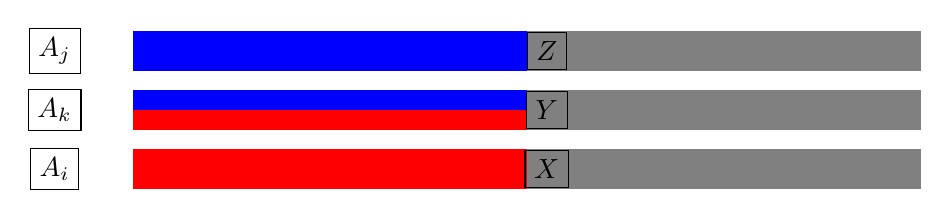
\begin{tikzpicture}
\node at (-1,0.25) [draw] {$A_i$};
\fill [gray]  (0,0) rectangle (10, 0.5);

\fill [red, very thick] (0,0) rectangle (5, 0.5);

\node at (5.25, 0.25) [draw] {$X$};

\node at (-1,1) [draw] {$A_k$};
\fill [gray]  (0,0.75) rectangle (10, 1.25);

\fill [red, very thick] (0, 0.75) rectangle (5, 1);
\fill [blue, very thick] (0,1) rectangle (5, 1.25);

\node at (5.25, 1) [draw] {$Y$};

\node at (-1,1.75) [draw] {$A_j$};
\fill [gray]  (0,1.5) rectangle (10, 2);

\fill [blue, very thick] (0, 1.5) rectangle (5, 2);

\node at (5.25, 1.75) [draw] {$Z$};
\end{tikzpicture}
\end{figure}

已知$X \neq Y$且$Y \neq Z$。由于字典序$A_i < A_k < A_j$,因此$X < Y < Z$,故$X \neq Z$,因此结论依然成立。
\end{block}
    
\end{frame}

\begin{frame}{Height数组}
    
\begin{block}{Height数组}

$Height[i]$为后缀$i$与排名在他前面一个的后缀的LCP,即:
$Height[i] = LCP(S[i, n], S[sa[rk[i]-1], n])$。

有了$Height[i]$数组之后,利用上一节的性质,任意两个后缀的LCP就变为区间最小值查询。

\pause
如何求$Height$呢?

\end{block}
\end{frame}


\begin{frame}{求Height数组}
    
\begin{block}{Height数组}
结论:$Height[i] \geq Height[i-1] -1$。

证明:
\pause
\begin{figure}
    \centering
    
\includegraphics[width=0.95\textwidth]{./emo.png}
\end{figure}

\end{block}    

\end{frame}

\begin{frame}{证明 $Height[i] \geq Height[i-1] -1$}
    
\begin{block}{1. 若$Height[i-1] \leq 1$}
$Height[i-1] = LCP(S[i-1, n], S[{\color{red}K1 =}sa[rk[i-1]-1], n])$。

$Height[i] = LCP(S[i, n], S[{\color{red}K2 = }sa[rk[i]-1], n])$。

1. 显然,$Height[i-1] = 1 / 0$,则结论$Height[i] \geq 0$成立。

\end{block}
\end{frame}

\begin{frame}{证明 $Height[i] \geq Height[i-1] -1$}

\begin{block}{2. 若$Height[i-1] > 1$}

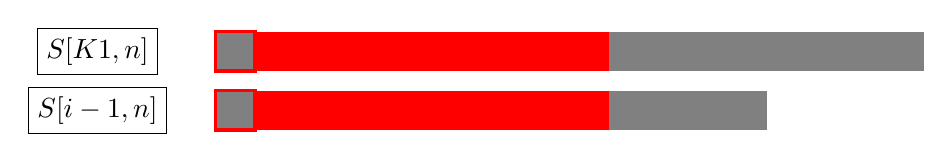
\begin{tikzpicture}
\node at (-1.5,0.25) [draw] {$S[i-1, n]$};
\fill [gray]  (0,0) rectangle (7, 0.5);

\fill [red, very thick] (0.5,0) rectangle (5, 0.5);
\draw [red, very thick] (0,0) rectangle (0.5, 0.5);

\node at (-1.5,1) [draw] {$S[K1,n]$};
\fill [gray]  (0,0.75) rectangle (9, 1.25);

\fill [red, very thick] (0.5, 0.75) rectangle (5, 1.25);

\draw [red, very thick] (0,0.75) rectangle (0.5, 1.25);
\end{tikzpicture}

\pause
则去掉首字母后,红色部分依然相等,且字典序关系不变。

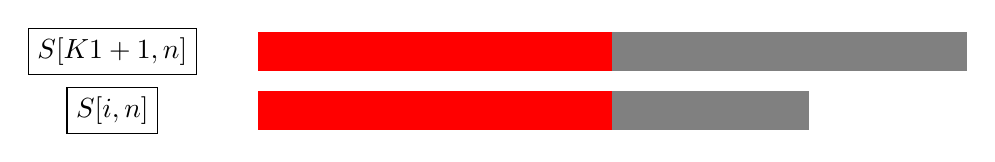
\begin{tikzpicture}
\node at (-1.85,0.25) [draw] {$S[i,n]$};
\fill [gray]  (0,0) rectangle (7, 0.5);

\fill [red, very thick] (0,0) rectangle (4.5, 0.5);

\node at (-1.85,1) [draw] {$S[K1 + 1, n]$};
\fill [gray]  (0,0.75) rectangle (9, 1.25);

\fill [red, very thick] (0, 0.75) rectangle (4.5, 1.25);

\end{tikzpicture}

即:$S[K1+1, n] < S[i,n]$,且$LCP(S[K1+1, n], S[i,n]) = Height[i-1] - 1$。

由于$S[K1+1, n] \leq S[K2,n] < S[i,n]$,因此应用“区间可加性”:

\begin{aligned}
Height[i-1] - 1 &= LCP(S[K1+1,n], S[i,n]) \\
&= min(LCP(S[K1+1, n], S[K2, n]), LCP(S[K2,n], S[i,n])) \\
&= min(LCP(S[K1+1, n], S[K2, n]), Height[i])
\end{aligned}

因此结论成立。

\end{block}
\end{frame}

\begin{frame}{求Height数组}

\begin{block}{求Height}
首先让$Height[i]$继承$Height[i-1] - 1$,然后向后暴力延申。

利用势能分析,易得:势能增长量 = 势能减少量 = $O(n)$。

\textbf{实际使用时常令$H[i] = Height[sa[i]]$($H[rk[i]] = Height[i]$),$H[i]$表示排名为$i$与$i-1$的串的LCP。}
\end{block}

\end{frame}

\begin{frame}{模板题}
    
\begin{block}{\href{https://www.luogu.com.cn/problem/P3809}{某谷3809}}
给出一个字符串,按字典序大小输出后缀位置。
\end{block}
\end{frame}

\begin{frame}{Height应用:求本质不同子串}
    
\begin{block}{\href{https://www.spoj.com/problems/SUBST1/}{SPOJ SUBST1}}
给出一个字符串,长度不超过$50,000$,求本质不同子串数量。
\end{block}

\pause

\begin{block}{题解}
答案 = $\sum{n - sa[i] + 1 - H[i]}$。
\pause

按字典序从小到大枚举所有后缀,统计有多少个新出现的前缀即可。

对于排名第$i$的后缀$S[sa[i],n]$,共有$n - sa[i] + 1$个前缀,其中有$H[i]$个前缀同时出现在前一个排名的后缀$S[sa[i-1], n]$中,因此减掉即可。

\pause

\textbf{上述证明是不完整的},还需要证明所有在$S[sa[i],n]$中出现,但没有在$S[sa[i-1],n]$中出现的前缀,他们在所有更小排名的后缀串也都没有出现。

\pause
\begin{figure}
    \centering
    
\includegraphics[width=0.7\textwidth]{./emo.png}
\end{figure}


\end{block}
\end{frame}

\begin{frame}{例题1}
    
\begin{block}{\href{https://ac.nowcoder.com/acm/problem/17141}{牛客17141}}
给出一个字符串,只由abc三种字母构成,求有多少置换意义下本质不同子串。

如果两个串在\{a,b,c\}的某种置换作用下相等,则认为是本质相同串。
\end{block}

\pause

\begin{block}{题解}
由于字符集很小,可以枚举所有的6种置换,于是每种本质不同子串都会出现6种不同的版本。

\pause

然而有一个例外是:如果是全a(b/c)串,则在6种置换的作用下,只会出现3个不同版本。

因此本题需要统计本质不同子串,以及本质不同的全a(b/c)串。

\pause

可以将6个置换串,用互不相同的连接符(例如:'z'+1到'z'+5)首尾拼接,求出cntA为本质不同全a(b/c)串个数,cntB为至少包含两种不同字母的本质不同串(且不包含连接符)。

答案 = $\frac{cntA}{3} + \frac{cntB}{6}$。

\end{block}
\end{frame}

\begin{frame}{例题2}

\begin{block}{\href{http://poj.org/problem?id=3415}{POJ3415}}
给出两个字符串S和T,求有多少个长度大于K的公共子串(区间)。
\end{block}
    
\pause

\begin{block}{题解}
用特殊字符连接两个串,进行后缀排序,得到$H$数组。

于是问题转化为对于所有区间$[l,r]$,求$max(0, min(H[l..r]) - K)$的和。从左到右扫描维护单调栈,或者分治,或者离线数据结构都可。
\end{block}
\end{frame}


\begin{frame}{例题3}
    
\begin{block}{题意}

给出两个串$S$和$T$,求最长公共子串长度。

\end{block}

\pause

\begin{block}{题解}
用特殊字符连接两个串,进行后缀排序,得到$H$数组。

求每一个$T$的后缀与所有的$S$后缀的最大LCP,取最大值即为答案。

枚举每个属于$T$的后缀,向左向右寻找第一个属于$S$的后缀$S_l$和$S_r$,求所有$max(LCP(T,S_l), LCP(T,S_r))$的最大值即可。
\end{block}
\end{frame}
\begin{frame}{例题4}

\begin{block}{题意}
给出两个字符串S和T,求有多少\textbf{本质不同}公共子串。
\end{block}
    
\pause

\begin{block}{题解}
用特殊字符连接两个串,进行后缀排序,得到$H$数组。

从左到右扫描属于$T$串的后缀,用上题的放法求每个$T$串的后缀与所有$S$串后缀的最大LCP,记为$MXLen$。

由于需要统计本质不同,需要找到前一个排名的属于$T$串的后缀,求出他们的LCP用于去重,记为$MNLen$。

则答案 = $\sum{MXLen - MNLen}$
\end{block}
\end{frame}

\begin{frame}{例题5}

\begin{block}{\href{https://ac.nowcoder.com/acm/problem/233969}{WF 2019 First of Her Name}}

给出一棵反向的Trie树,每个点表示一个人的名字:从该点走到根边上的字符首尾拼接形成。

有若干次询问,每次询问给出一个字符串,问他是多少个人名字的前缀。
\end{block}
    
\pause

\begin{block}{题解}
之前讲过离线AC自动机的做法,今天讲在线树上SA的做法。

\pause

普通的SA是排序一个字符串的所有后缀,树上SA则是排序所有Trie树节点表示的字符串。

\pause

排序原理完全一样:使用ST表进行倍增+基数排序。

\pause

回答询问时,进行暴力二分求lower\_bound和upper\_bound即可。

复杂度$O(\Sigma \log{n})$。
\end{block}
\end{frame}
\end{document}	% Done!